\subsection{Типы измерений}

Для уточнения орбиты требуются измерения параметров, связанных с положением и движением КО.
Конкретный набор измеряемых параметров зависит от типа используемых наблюдательных средств.
Далее приведены несколько стандартных наборов измеряемых величин и примеры их технической реализации.

\subsubsection{Односторонние измерения дальности}
Расстояние между спутником и станцией наблюдения является одним из наиболее часто измеряемых параметров.
Такая модель измерений получила широкое распространение во многом благодаря глобальным навигационным спутниковым системам.
Каждый спутник ГНСС оснащен антенной, которая излучает электромагнитные волны на нескольких частотах.
Сигнал каждого спутника модулируется особым образом, чтобы приемник мог определить момент времени $T_{T}$ излучения волны по шкале времени спутника
и соответствующие этому моменту координаты излучателя. Момент приема сигнала $T_{R}$ фиксируется по часам приемника.

Зная разницу между временем отправки и приема сигнала, а также используя свойство прямолинейности распространения света, можно 
рассчитать величину, называемую псевдодальностью:
\begin{equation*}
    \rho = (T_{R} - T_{T}) c,
\end{equation*}
где $c$ -- скорость света.

Псевдодальность не совпадает с геометрической в силу несогласованности часов излучателя и приемника, 
особенностей распространения сигнала в атмосфере и относительного движения излучателя и приемника.

Учет этих факторов необходим при формировании расчетного аналога измерения:

\begin{equation*}
    \tilde{\rho} = |\vec{r}_{T} - \vec{r}_{R}| 
                    + c \left( \delta t_{T} - \delta t_{R} \right)
                    + \delta \rho_{tropo} + \delta \rho_{ion} + \epsilon,
\end{equation*}
где помимо геометрической дальности $|\vec{r}_{T} - \vec{r}_{R}|$ присутствуют слагаемые,
связанные с поправкой часов спутника $\delta t_{T}$ и станции $\delta t_{R}$, тропосферная $\delta \rho_{tropo}$ и ионосферная $\delta \rho_{ion}$ задержки.
Благодаря измерениям на нескольких частотах ионосферная задержка может быть с высокой точностью исключена.
В $\epsilon$ включаются остаточные ошибки, связанные с неучитываемыми нелинейными эффектами.

Для повышения точности позиционирования и уменьшения разброса результатов
в ходе решения навигационной задачи могут обрабатываться не только псевдодальности,
но и фазовые измерения сигнала. 
В этом случае точность позиционирования с использованием ГНСС может достигать 10 сантиметров.

\subsubsection{Двусторонние измерения дальности}
В ходе двустороннего измерения дальности фиксируется время, за которое излученный сигнал
достигает цели, отражается и возвращается в точку испускания. 
Вариантом такой измерительной системы является лазерная дальнометрия (SLR).
В отличии от односторонних измерений дальности в лазерной дальнометрии излучатель и приемник
находятся в одном месте и подключены к одним часам, что избавляет от необходимости уточнения поправок шкал времени.
При этом атмосферные поправки все еще требуются. 
В качестве измерений усредняется расстояние, пройденное сигналом в прямом и обратном направлениях:

\begin{equation*}
    \rho_{avg} = \frac{1}{2} \left[ 
        \left(T_{R} - T_{T}\right) c + \delta \rho_{atm} + \epsilon \right]
\end{equation*}

Современные станции SLR используют лазеры с длиной волны 532 нм, что соответствует оптическому диапазону.
С этим связан недостаток лазерной дальнометрии -- зависимость от погодных условий.

В качестве примера применения SLR рассмотрим серию аппаратов LAGEOS (LAser GEOdynamics Satellite).
Аппараты LAGEOS-I и LAGEOS-II были запущены на среднюю околоземную орбиту в 1976 и 1992 годах соответственно.
Цель миссии -- изучение геодинамики, в частности, определение формы земной поверхности и уточнение параметров вращения Земли. 
Каждый аппарат имеет шарообразную форму и оснащен набором уголковых отражателей, необходимых
для точного отражения лазерного сигнала.

Позиционирование спутников выполняется на основе измерений наблюдательных пунктов Международной службы лазерной дальнометрии.
Ошибки лазерных измерений составляют менее 1 сантиметра, что позволяет восстанавливать орбиту аппаратов с точностью до нескольких сантиметров.

\subsubsection{Измерения дальности и радиальной скорости}
В некоторых случаях наблюдательные средства позволяют измерить не только
некоторый параметр движения, но и скорость его изменения. 
Так, производная дальности -- радиальная скорость, может быть получена из допплеровского сдвига.
Эффект Допплера заключается в частотном смещении, которое приобретает сигнал, принимаемый на движущемся объекте (или отраженный от движущегося объекта).
Величина смещения зависит от проекции относительной скорости излучателя и приемника на линию распространения сигнала,
то есть от радиальной скорости:

\begin{equation*}
    \Delta f_D = \frac{2 v_r f_t}{c},
\end{equation*}
где $v_r$ -- радиальная скорость, $f_t$ -- рабочая частота излучателя, $c$ -- скорость света.

Представителем данного класса систем является DORIS,
которая обеспечивает измерение радиальной скорости с точностью до 0.5 мм/с.
В состав комплекса DORIS входят наземные маяки и космические аппараты, 
оборудованные соответствующими допплеровскими приемниками. 
В частности, Европейское космическое агентство 
использует DORIS для определения орбиты аппарата Cryosat-2, 
созданного с целью измерения толщины ледового покроя.

\subsubsection{Угловые измерения}

Для описания угловых измерений рассмотрим несколько дополнительных систем координат.

Форма Земли может быть приближенно представлена в виде опорного эллипсоида.
В силу несферичности земной поверхности локальная вертикаль не совпадает с направлением на центр Земли, определяемым сферическими координатами.
Поэтому сферическая СК неудобна при проведении измерений 
и вводится геодезическая СК (рис. \ref{fig:geodes}), привязанная к опорному эллипсоиду.
В этой системе широта и долгота определяют направление на зенит.

\begin{figure}[h!]
    \centering
    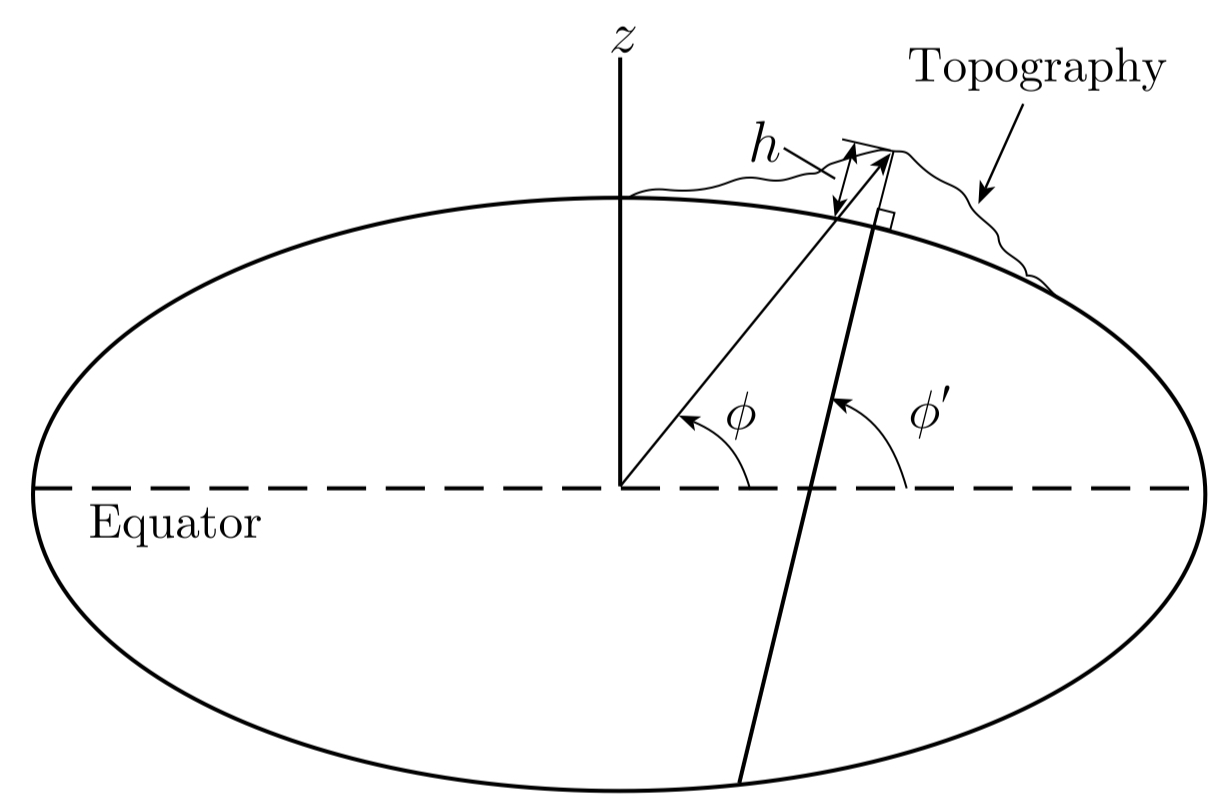
\includegraphics[width=0.5\linewidth]{../images/review/geodes.PNG}
    \captionof{figure}{Геодезическая система координат. 
    $\phi$ -- геодезическая широта,
    $h$ -- высота над опорныи эллипсоидом}
    \label{fig:geodes}
\end{figure}

Для координатного описания локальной области на поверхности эллипсоида
применяется топоцентрическая СК (рис. \ref{fig:topo}). Это декартова система, начало которой привязано к некоторой точке на эллипсоиде,
а оси сонаправлены касательным координатных линий топоцентрической СК в данной точке.

\begin{figure}[h!]
    \centering
    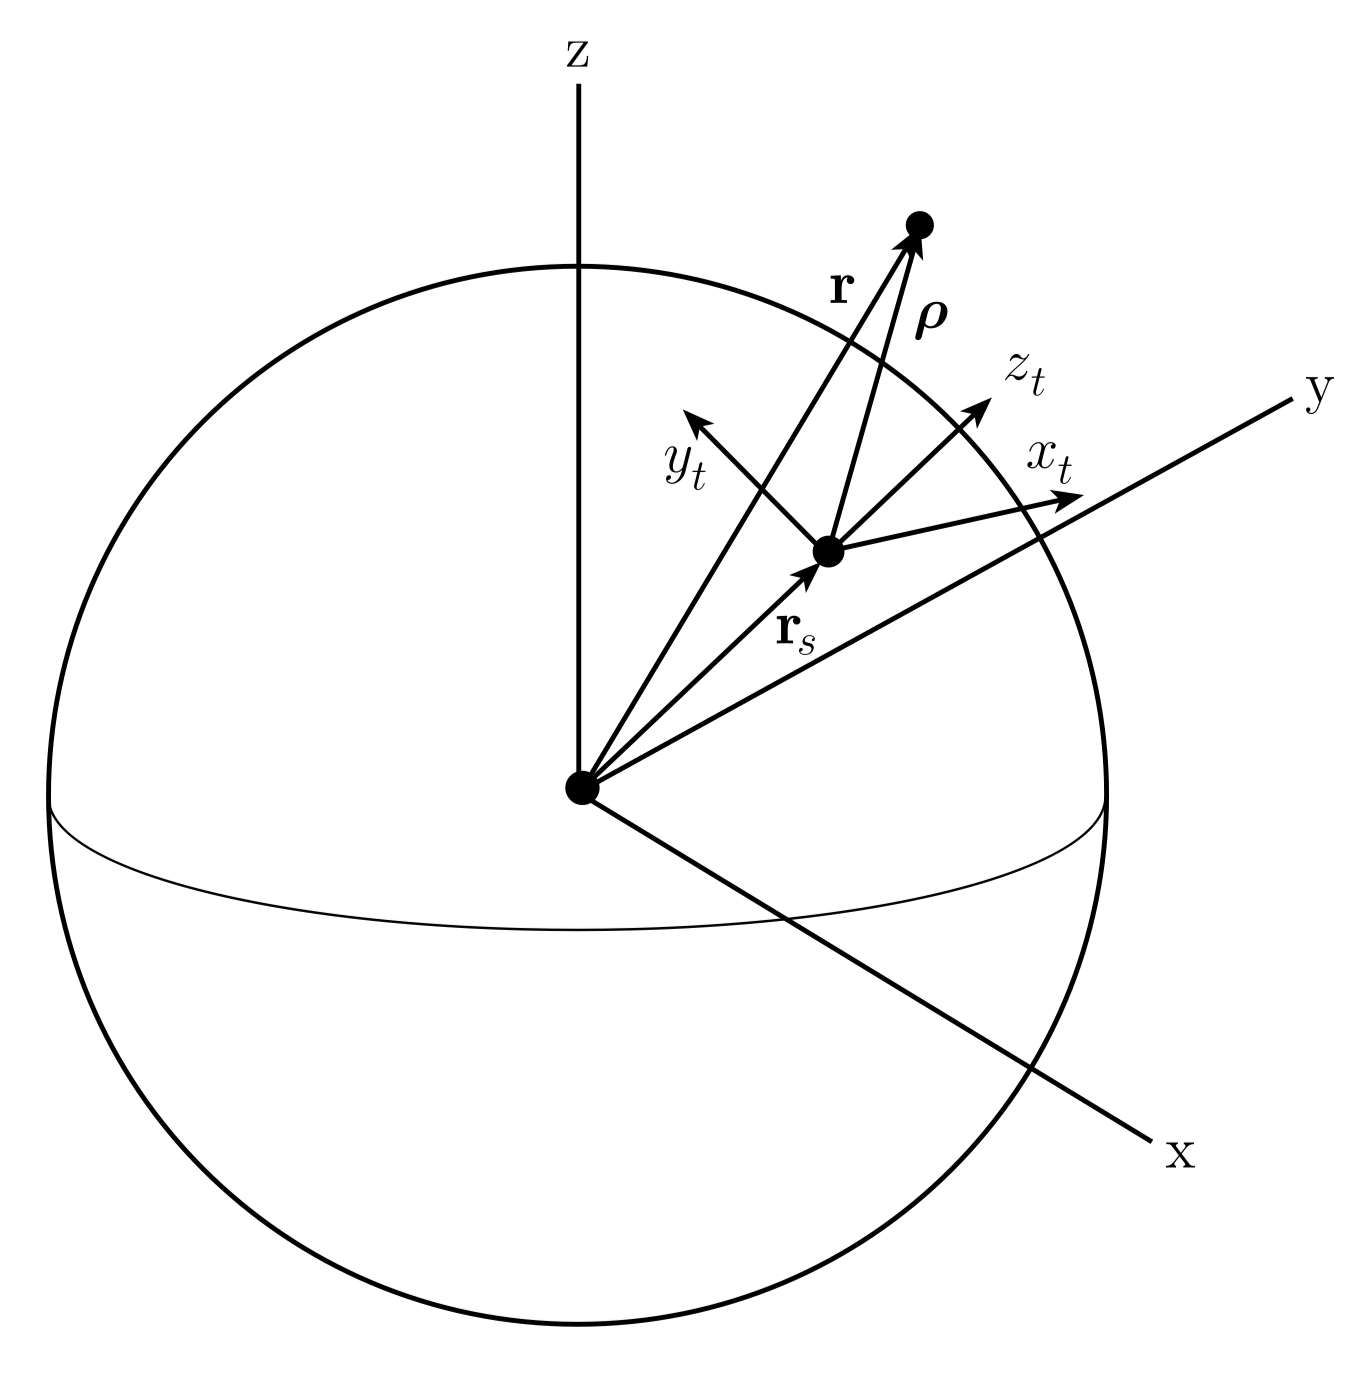
\includegraphics[width=0.5\linewidth]{../images/review/topo.PNG}
    \captionof{figure}{Топоцентрическая система координат.
    $x, y, z$ -- оси исходной СК, \\
    $x_t, y_t, z_t$ -- оси локальной СК}
    \label{fig:topo}
\end{figure}

Направление в локальной системе координат можно описать с помощью
азимута и угла возвышения (рис. \ref{fig:enu}).
Именно эти углы используются для ориентации наблюдательных средств.
Затем на начальном этапе обработки измерений набор локальных углов
может быть пересчитан в долготу и широту в сферической системе координат.

\begin{figure}[h!]
    \centering
    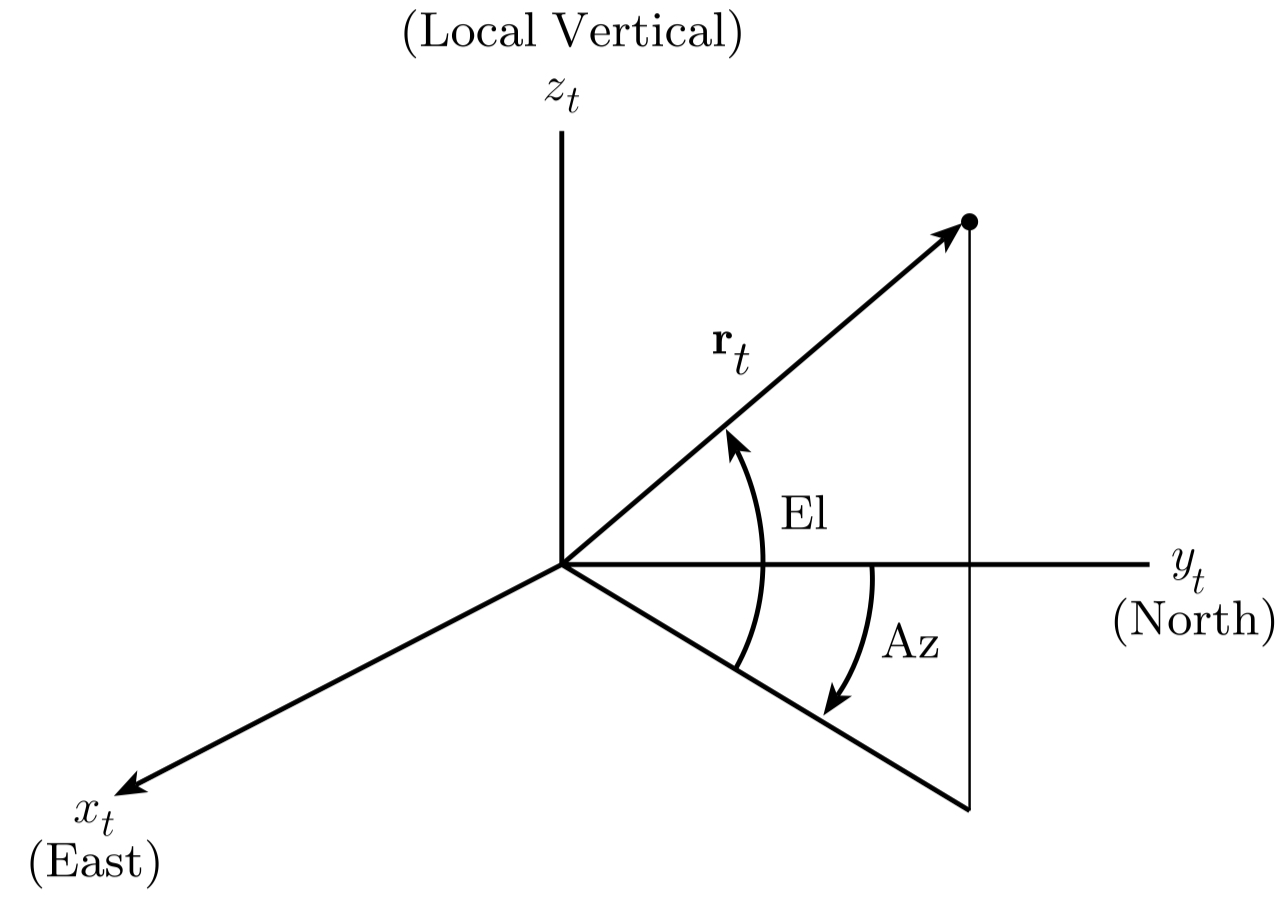
\includegraphics[width=0.5\linewidth]{../images/review/enu.PNG}
    \captionof{figure}{Локальная система координат. \\
    Az -- азимут, отсчитывается от направления на север \\
    El -- угол возвышения, отсчитывается от плоскости поверхности}
    \label{fig:enu}
\end{figure}

Техническая реализация угловых измерений зачастую связана с оптическими инструментами. 
Классическим примером таких инструментов являются телескопы. 
В первом приближении методика получения угловых измерений с помощью телескопа достаточно проста.

Телескоп с закрепленной на объективе фотокамерой направляется на интересующий участок неба.
Затем открывается затвор камеры и снимок неба экспонируется в течение заданного промежутка времени.
Для компенсации движения звезд на небесной сфере при длинных выдержках крепления телескопа
оснащаются приводами. Это позволяет сохранить фиксированную ориентацию относительно звездной системы координат.
В то же время проекция траектории космического объекта на небесную сферу представляет собой линию -- трек.
Зная угловые координаты звезд (например, из звездного каталога), можно определить угловые координаты объекта во время пролета.

В настоящее время для контроля околоземного пространства также повсеместно применяются активные радиолокаторы.
Локатор состоит из набора излучателей, испускающих сигнал и приемников, фиксирующих отраженный от объекта сигнал.
Зона обзора для барьерных РЛС двумерная (сектор), а для обзорных РЛС объемная (усеченная пирамида).
Применение в локаторах активной фазированной антенной решетки позволяет определять не только расстояние и 
радиальную скорость, но и направление на объект.